\documentclass{scrartcl}

\usepackage[utf8]{inputenc}
\usepackage{color}
\usepackage{xcolor}

\usepackage{graphics}           % Add pictures to the document
\usepackage{graphicx}           % Add pictures to the document
\usepackage{subfigure}          % 2 pictures side by side

\title{Dokumentation ProductAR}
\author{Maximilian Rehberger}
\date{\today}

\setcounter{secnumdepth}{4}
\setcounter{tocdepth}{4}

\definecolor{darkcerulean}{rgb}{0.03, 0.27, 0.49}
\definecolor{frenchblue}{rgb}{0.0, 0.45, 0.73}
\definecolor{babyblueeyes}{rgb}{0.63, 0.79, 0.95}

\addtokomafont{section}{\color{darkcerulean}}
\addtokomafont{subsection}{\color{frenchblue}}
\addtokomafont{subsubsection}{\color{babyblueeyes}}

\graphicspath{ {./img/} }                % Path to images

\begin{document}


\maketitle

\newpage


\renewcommand*\contentsname{}
\section{Inhaltsverzeichnis}
\tableofcontents{}


\newpage

\section{Einleitung}

\subsection{Zweck}

Produkte können zum Beispiel beim Einkaufen mit dem Smartphone gescannt werden und erkannt werden. Informationen werden angezeigt wie zum Beispiel Bilder oder ein Preisvergleich. Mithilfe der App soll man einen Barcode einscannen können und Informationen zu den Produkten erhalten. Weiterhin kann der Nutzer ein Produkt in Augmented Reality (AR) testen und sieht somit wie es in Wirklichkeit aussehen wird, wenn er es kaufen würden.

\newpage

\section{Allgemeine Übersicht}

\subsection{Beschreibung Ausgangssituation}

Es gibt bereits viele Shopping-Apps wie zum Beispiel Ikea, H\&M oder S'Oliver. Das Problem ist, dass jeder am Ende für jedes Geschäft eine eigene App auf dem Smartphone hat. Diese App soll die Möglichkeiten geben mehrere unterschiedliche Produkte in einer App zu speichern und zu verwalten. Also eine App für alle Produkte.

\subsection{Produkteinsatz}

 Die App kann zum Beispiel als Einkaufsliste oder Wunschliste für Produkte eingesetzt werden.
 Darüber hinaus bieten sich noch viele weitere Möglichkeiten.

\subsection{Produktumfeld}

Die App wird hauptsächlich im privaten Umfeld umgesetzt, beim Einkaufen in Geschäften oder Online-Einkauf.

\subsection{Produktfunktionalität}

Scannen von Produkten, Informationen zu Produkten, Preisvergleich, Bilder hochladen für Produkte, Produkte in AR testen.

\subsection{Personas}

\subsubsection{Nutzer}

\subsubsection{Verkäufer}

\subsubsection{Admin}


\newpage

\section{Architekturkonzept und Entwurf}

\subsection{Ursprüngliches Architekturkonzept}

\begin{figure}[h]
\centering
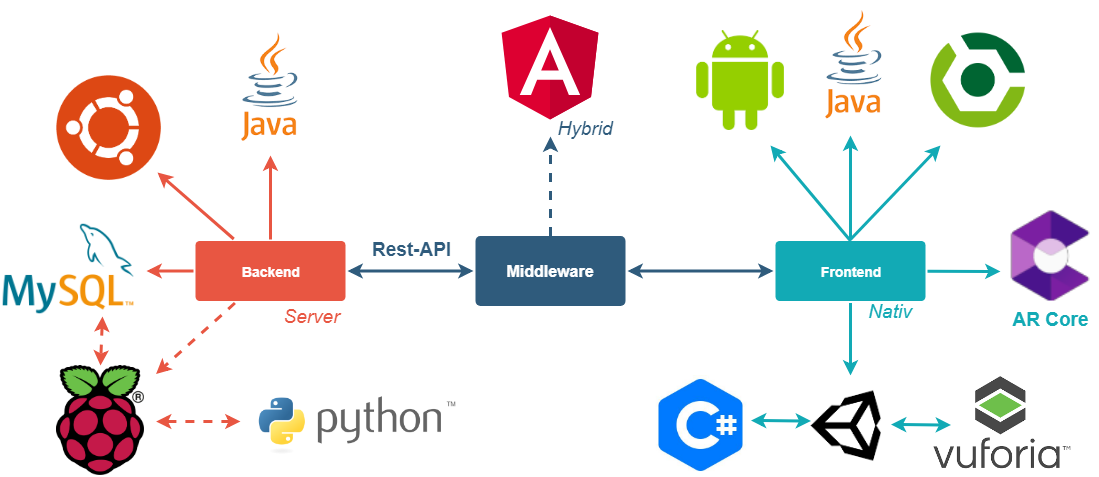
\includegraphics[width=380px]{img/Architekturkonzept.png}
\caption{Ursprüngliches Architekturkonzept}
\end{figure}

\subsection{Aktualisiertes Architekturkonzept}

\begin{figure}[h]
\centering
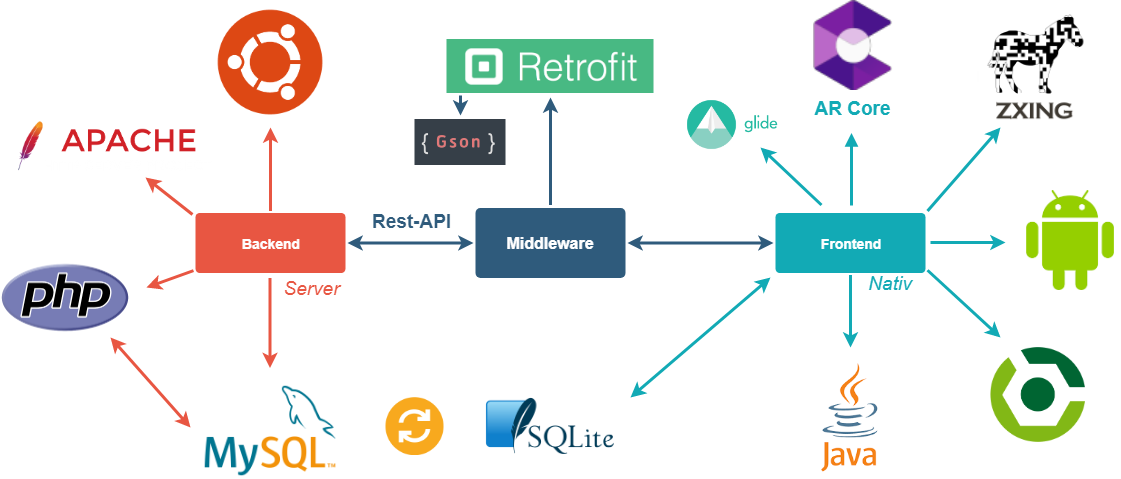
\includegraphics[width=380px]{img/ArchitekturkonzeptNew.png}
\caption{Aktualisiertes Architekturkonzept}
\end{figure}

\newpage

\subsection{Anfängliche Skizze Datenbankentwurf}

\subsubsection{MySQL Datenkbank (Remote)}

Ursprünglich war geplant, dass die Daten ausschließlich auf dem Server in einer MySQL Datenbank gespeichert werden.

\begin{figure}[h]
\centering
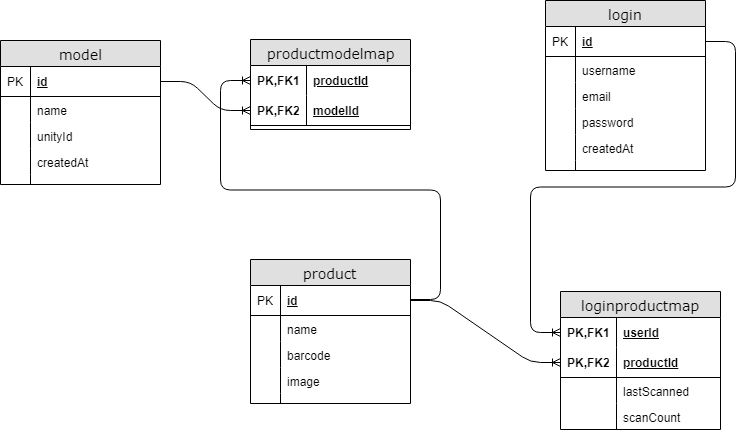
\includegraphics[width=380px]{img/Skizze_Datenbank_1.png}
\caption{Anfängliche Skizze Datenbankentwurf}
\end{figure}

\newpage

\subsection{Anfängliche Skizze Java Klassen}

\begin{figure}[h]
\centering
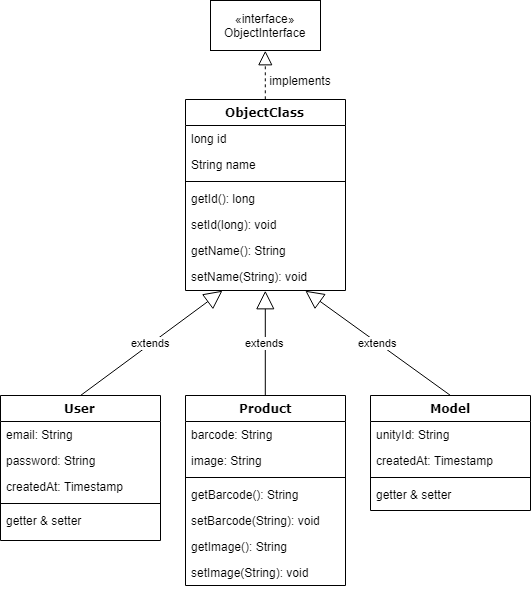
\includegraphics[width=320px]{img/Skizze_Java_1.png}
\caption{Anfängliche Skizze Datenbankentwurf}
\end{figure}

\newpage

\subsection{Endgültige Skizze Datenbankentwurf}

\subsubsection{SQLite Datenbank (Lokal)}

\begin{figure}[h]
\centering
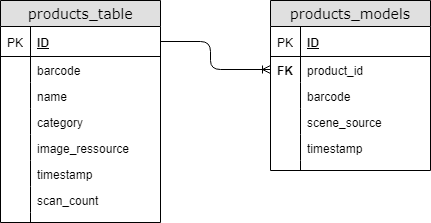
\includegraphics[width=180px]{img/Skizze_Datenbank_SQLite.png}
\caption{Skizze Datenbankentwurf: SQLite}
\end{figure}

\subsubsection{MySQL Datenbank (Remote)}

\begin{figure}[h]
\centering
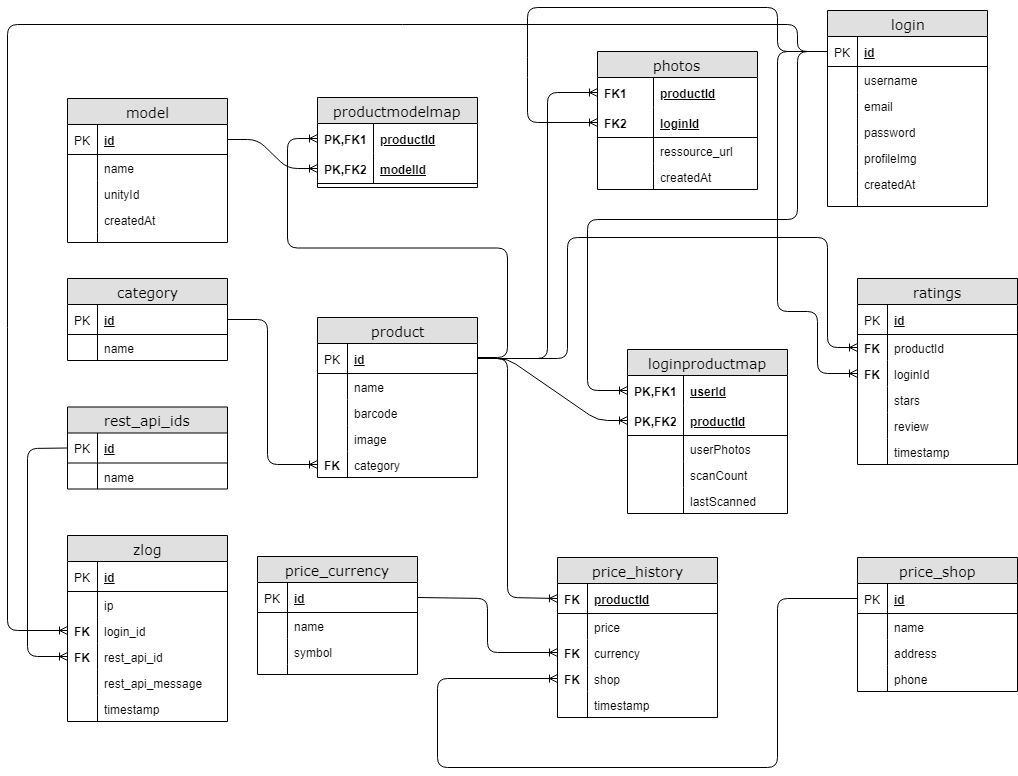
\includegraphics[width=380px]{img/Skizze_Datenbank_2.png}
\caption{Aktualisierte Skizze Datenbankentwurf: MySQL}
\end{figure}

\newpage

\subsection{Endgültige Skizze Java Klassen}

\begin{figure}[h]
\centering
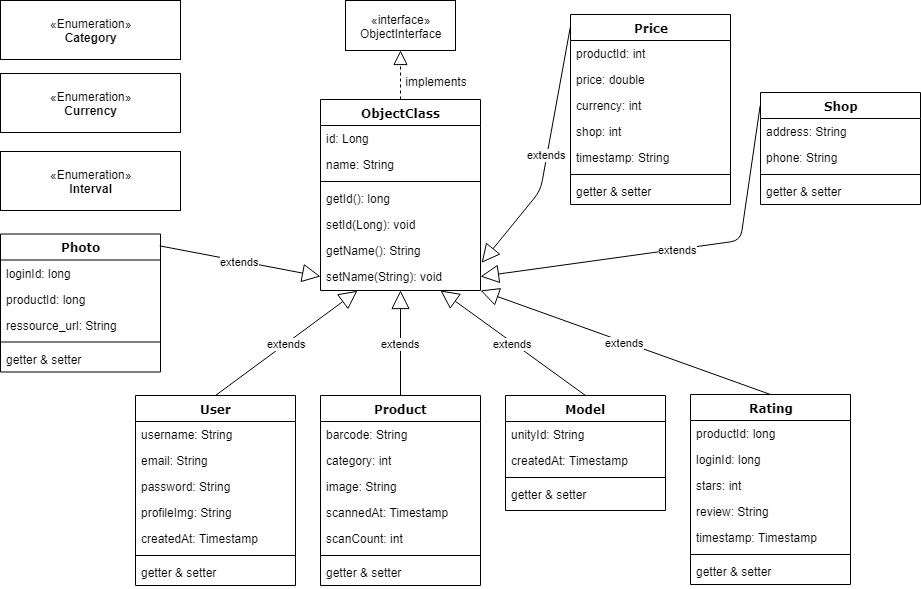
\includegraphics[width=380px]{img/Skizze_Java_New.png}
\caption{Aktualisierte Skizze: Java Klassen}
\end{figure}

\subsection{Übersicht Backend Server}

Der Backend Server ist ein gemieteter Server von Hosteurope. \newline
Produktbezeichnung: "Virtual Server Linux Advanced 8.2". \newline
Dieser hat folgende Linux Version installiert: Ubuntu 16.04.6 LTS. \newline \newline

\noindent Die Technischen Spezifikationen lauten wie folgt: \newline 

\noindent 4 virtuelle Kerne \newline
\noindent 6 GB RAM \newline 
\noindent 200GB SSD \newline 

\noindent Es handelt sich hierbei um einen virtuellen Server, das bedeutet, dass sich der Server mit anderen "Containern" die Hardware eines Servers teilen. % Die Hardware eines großen Server wird auf die Container entsprechend aufgeteilt. % 
\newline

\noindent Der Server hat eine eigene Domain: www.nimoo.de. 

\newpage

\subsection{Übersicht REST API}

Die Rest Schnittstelle wurde mit PHP auf dem Webserver umgesetzt welcher vom Backend Server bereits zur Verfügung gestellt wurde. 
Für jede Ressource existiert ein Pfad, mit entsprechender PHP Datei. \newline 

\noindent Der Hauptpfad für die App auf dem Webserver: "https://www.nimoo.de/apps/productar" \newline

\noindent Folgende Pfade existieren auf dem Webserver: \newline

\noindent ../products/ \newline
\noindent ../products/images/ \newline
\noindent ../products/photos/ \newline
\noindent ../products/prices/ \newline
\noindent ../products/ratings/ \newline
\noindent ../users/ \newline
\noindent ../users/images \newline
\noindent ../models/ \newline

\subsection{Technische Entscheidungen}

\subsubsection{Warum Android?}

Die Entscheidung, die App für Android zu entwickeln wurde getroffen, da Android zumindest in Deutschland einen höheren Marktanteil besitzt als iOS. Vor allem die Studenten der Fakultät Informatik und Wirtschaftsinformatik (FIW) und in der Vertiefung Mobile Solutions benutzen mehrheitlich Android Smartphones. Ein weiterer Grund ist, dass Android Java basiert ist und dafür sehr gut geeignet ist, wenn bereits fortgeschrittene Erfahrungen mit der Programmiersprache Java gegeben sind. Weiterhin gibt es beim Entwickeln keine Mehrkosten, da es bereits viele Open-Source Erweiterungen (Bibliotheken) gibt und Anleitungen, die das Entwickeln weiter vereinfachen.

\subsubsection{Welche Androidversion?}

Als minimal unterstützte Android Version (minSdkVersion) für die App musste die Api 24 (Android 7) verwendet werden. Dies liegt daran, dass die AR Funktionialität mit der Google AR Core Erweiterung erst ab Android Version 7 (Api 24) unterstützt wurde und alle vorherigen Versionen keine Unterstützung haben. Dies hat den Nachteil, dass nur ca. 37,1 \% aller Android Geräte unterstützt werden im Vergleich zu den 95,3 \% die mit Android 4.4 (Api 19) unterstützt würden. 

\subsubsection{Welche Entwicklungsumgebung?}

Zum Entwickeln der App wurde hauptsächlich die Entwicklungsumgebung von Android Studio und IntelliJ genutzt.

\subsubsection{Wieso Google AR Core?}

Googles neuestes Framework für Augmented Reality Anwendungen heist "AR Core". Im Vergleich zu einer AR Anwendung mit Unity lässt es es sich sehr einfach in die App integrieren (Als Fragment oder View in der Aktivity). Weiterhin lassen sich Modelle (.OBJ) sehr einfach mit dem Sceneform Plugin einbinden und bearbeiten. 

\subsubsection{Wieso eine MySQL Datenbank?}

Zum einen war die MySQL Datenbank ebenfalls schon auf dem Backend Server aufgesetzt, somit war keine weitere Konfiguration notwendig. Weiterhin ist es sehr einfach eine Datenbank mit SQL zu erstellen und Abfragen durchzuführen.

\subsubsection{Wieso eine REST API?}

Die Rest API ist die Schnittstelle zwischen der App und der Datenbank auf dem Server. Diese wird benötigt, da man aus Sicherheitsgründen keine direkte Verbindung zwischen App und Datenbank zulassen darf.

\subsubsection{Vergleich mit Alternativlösungen}

\paragraph{Firebase von Google}.\newline

\noindent Die Backendlösung von Google ist "FireBase" und wäre erheblich einfacher umzusetzten und hätte ebenfalls den Vorteil, dass kein externer Server benötigt wird. Warum wurde diese Lösung in diesem Projekt jedoch nicht verwendet? Die Datenbank enthält sensible Daten, wie zum Beispiel Nutzerdaten. Diese sollen nicht an Google gesendet werden.

\paragraph{Alternative Datenbankmodelle}.\newline

\noindent PostgreSQL und MongoDB.

\newpage

\section{Technische Dokumentation}

Die Dokumentation der einzelnen Java Klassen befindet sich im generierten JavaDoc Verzeichnis. Die nachfolgende Dokumentation wurde aus den JavaDoc Kommentaren übernommen. Bestimmte Klassen können doppelt vorkommen.

\subsection{Android Manifest}

\subsection{Java Interfaces}

\subsubsection{ObjectInterface}

Das Interface "ObjectInterface" definiert die Vorgaben, welches ein Objekt erfüllen muss. Ein Objekt benötigt eine id als eindeutigen Identifizierer und einen Namen. Entsprechende Getter und Setter sind hier definiert.

\subsubsection{ScanResultReceiver}

Das Interface "ScanResultReceiver" definiert die Methoden, welche nach dem Scannen eines Barcodes ausgeführt werden. \newline

\noindent\textbf{Methode scanResultData(NoScanResultException noScanData)}\newline Die Methode "scanResultData" wird aufgerufen, wenn das Scannen des Barcodes fehlgeschlagen ist.\newline

\noindent\textbf{Methode scanResultData(java.lang.String codeFormat, java.lang.String codeContent)}\newline Die Methode "scanResultData" wird nach dem erfolgreichen Scannen des Barcodes aufgerufen.

\subsubsection{IRetrofitCRUD}

Das Interface "IRetrofitCRUD" definiert die Methoden, welche aufgerufen werden um über Retrofit Anfragen an den Server zu stellen.

\subsubsection{JsonPlaceHolderApi}

Das Interface "JsonPlaceHolderApi" ist die direkte Schnittstelle zwischen Retrofit und dem Zielserver. Verwendete HTTP Verbs: GET und POST.

\subsection{Java Klassen}

\subsubsection{Objekt Klassen}

\paragraph{Object Class (Abstract)}

Die Klasse "ObjectClass" ist eine abstrakte Klasse, welche die benötigten Methoden für ein Objekt implementiert.

\paragraph{Product}

Die Klasse "Product" stellt die Objektklasse für ein Produkt dar. Ein Produkt ist gleichzeitig ein Objekt. Hier werden wichtige Methoden und Konstruktoren implementiert. Die Werte können über Getter und Setter Methoden abgefragt werden.

\paragraph{User}

Die Klasse "User" stellt die Objektklasse für einen Benutzer dar. Ein Benutzer ist gleichzeitig ein Objekt. Hier werden wichtige Methoden und Konstruktoren implementiert. Die Werte können über Getter und Setter Methoden abgefragt werden.

\paragraph{Model}

Die Klasse "Model" stellt die Objektklasse für ein (AR) Model dar. Ein Model ist gleichzeitig ein Objekt. Hier werden wichtige Methoden und Konstruktoren implementiert. Die Werte können über Getter und Setter Methoden abgefragt werden.

\paragraph{Photo}

Die Klasse "Photo" stellt die Objektklasse für ein Foto dar. Ein Foto ist gleichzeitig ein Objekt. Hier werden wichtige Methoden und Konstruktoren implementiert. Die Werte können über Getter und Setter Methoden abgefragt werden.

\paragraph{Price}

Die Klasse "Price" stellt die Objektklasse für einen Preis dar. Ein Preis ist gleichzeitig ein Objekt. Hier werden wichtige Methoden und Konstruktoren implementiert. Die Werte können über Getter und Setter Methoden abgefragt werden.

\paragraph{Shop}

Die Klasse "Shop" stellt die Objektklasse für einen Shop dar. Ein Shop ist gleichzeitig ein Objekt. Hier werden wichtige Methoden und Konstruktoren implementiert. Die Werte können über Getter und Setter Methoden abgefragt werden.

\paragraph{Category (Enum)}

Die Enumklasse "Category" beinhaltet die Produktkategorien. Es gibt folgende Kategorien: Accessoires, Auto, Baumarkt, Beauty, Bücher, Computer, Drogerie, Elektronik, Filme, Garten, Haushalt, Kleidung, Lebensmittel, Möbel, Musik, Schuhe, Serien, Spiele, Spielzeug, Sport.

\paragraph{Currency (Enum)}

Die Enumklasse "Currency" beinhaltet die aktuell unterstützten Währungen. In diesem Fall: Dollar und Euro.

\paragraph{Interval (Enum)}

Die Enumklasse "Interval" beinhaltet die Möglichkeiten für ein Updateinterval der Benachrichtigungen. Folgende Intervalle sind für Benachrichtigungen möglich: Täglich, Wöchentlich, Monatlich.

\newpage

\subsubsection{Aktivity Klassen}

\paragraph{MainActivity}

\noindent Die Klasse "MainActivity" wird beim Starten der App ausgeführt, direkt nach dem "SplashScreen". Es können Barcodes gescannt und danach das Ergebnis angezeigt werden.\newline

\noindent\textbf{Methode onCreate(android.os.Bundle savedInstanceState)}

\noindent Die Methode "onCreate" wird beim Start der Activity ausgeführt. Hier werden Werte initialisiert, zum Beispiel TextViews oder Buttons. Es wird eine Datenbankverbindung zur lokalen SQLite Datenbank initialisiert. Ein OnClickListener wird für den Button "btn\_scan\_now" initialisiert. Für Android Versionen größer 23 (ab 24) wird ein NetworkMonitor Receiver erzeugt.\newline

\noindent\textbf{Methode onCreateOptionsMenu(android.view.Menu menu)}

\noindent Die Methode "onCreateOptionsMenu" erzeugt das Menü für die AktionsLeiste Es wird zuerst überprüft ob der Nutzer eingeloggt ist. Nutzername und Password werden in einem User Objekt gespeichert. Das Menü "menu\_loggedin" wird hier verwendet. Der Nutzername wird in das Feld "action\_username" eingetragen und ein OnClickListener erstellt mit der Methode "goToProfile". Für den Logout Button wird ebenfalls ein OnClickListener erstellt, welcher den Nutzer ausloggt. Ist der Nutzer allgemein nicht eingloggt, so wird stattdessen das Standardmenü geladen. \newline

\noindent\textbf{Methode onDestroy()}

\noindent Die Methode "onDestroy" wird beim verlassen der Activity ausgeführt. \newline

\noindent\textbf{Methode onOptionsItemSelected(android.view.MenuItem item)}

\noindent Die Methode "onOptionsItemsSelected" wird ausgeführt, wenn ein Menüelement ausgewählt wurde. Je nachdem um welches Element es sich handelt werden unterschiedliche Aktionen ausgeführt. Bei "action\_login": Wenn eingeloggt, dann wird mann zum Profil weitergeleitet. Wenn nicht eingeloggt, dann wird man zum Login weitergeleitet. Bei "action\_settings": Man wird zu den Einstellungen weitergeleitet. Bei "action\_info": Man wird zu den Informationen über die App weitergeleitet. Bei "action\_close": Die App wird beendet. \newline

\noindent\textbf{Methode scanNow(android.view.View view)}

\noindent Die Methode "scanNow" wird ausgeführt, wenn der Button "btn\_scan\_now" geklickt wurde. Es wird ein ScanFragment erzeugt, welches als nächstes geöffnet wird. Die Kamera wird aktiviert und der Barcode Scanner wird initialisiert. \newline

\noindent\textbf{Methode scanResultData(java.lang.String codeFormat, java.lang.String codeResult)}

\noindent Die Methode "scanResultData" wird ausgeführt, wenn der Barcode Scanner einen Code erfolgreich gescannt hat. Zuerst wird geprüft ob der barcode existiert (!nullCheck) Als nächstes beginnt die Ladeanimation (loadingStart()) Es wird versucht den Barcode in eine Long Variable umzuwandeln um zu prüfen ob der Barcode numerisch ist. Wenn keine NumberFormatException abgefangen worden ist wird in der lokalen SQLite Datenbank nach einem Barcode gesucht, welcher schon existiert. Von diesem wird der Name und das Bild benötigt. Wenn kein Barcode lokal existiert, dann wird eine Abfrage mit Retrofit ausgeführt, welche prüft ob ein Produkt mit dem Barcode in der MySQL Datenbank auf dem Server vorhanden ist. Sollte ein Produkt auf dem Server existieren, dann wird es in die Lokale Datenbank übertragen Es wird zusätzlich überprüft ob ein Model zu dem Produkt in der lokalen Datenbank existiert, wenn nicht, dann wird eins vom Server angefragt und in die Datenbank übertragen. Wenn kein Produkt auf dem Server existiert, dann wird die Methode "createNewBarcode" aufgerufen um einen neues Produkt auf dem lokalen Gerät zu erstellen. Wenn der Barcode bereits lokal existiert, wird der Zeitstempel für das Produkt aktualisiert und die Anzahl der Scans um 1 inkrementiert. Außerdem wird das Produkt als "bereit zum Synchronisieren" gekennzeichnet Das Ergebnis für das Bild und den Namen aus der lokalen Datenbank wird nun angezeigt und in die davor vorgesehenen Views geladen. Abschließend wird die Ladeanimation wieder beendet (loadingEnd()) \newline

\noindent\textbf{Methode scanResultData(NoScanResultException noScanData)}

\noindent Für den Fall das der Scan fehlgeschlagen ist. \newline

\noindent\textbf{Methode createNewBarcode(java.lang.String newBarcode)}

\noindent Die Methode "createNewBarcode" leitet auf die "CreateProductActivity" weiter und übergibt dieser den gescannten Barcode. \newline

\noindent\textbf{Methode goToProfile()}

\noindent Die Methode "goToProfile" leitet einen zum Nutzerprofil weiter. \newline

\noindent\textbf{Methode loadingStart()}

\noindent Die Methode "loadingStart" startet die Ladeanimation. \newline

\noindent\textbf{Methode loadingEnd()}

\noindent Die Methode "loadingEnd" beendet die Ladeanimation. \newline

\newpage

\paragraph{SplashScreen}

Die "SplashScreen" Activity wird ganz am Anfang gestartet. Es wird ein Drawable angezeigt. Anschließend wird auf die "MainActivity" weitergeleitet. \newline

\noindent\textbf{Methode onCreate(android.os.Bundle savedInstanceState)}

\noindent Die Methode "onCreate" initialisiert Variablen und ruft die Methode "scheduleJob" auf. Weiterhin wird ein CountdownTimer eingestellt, welcher beim Ablauf auf die "MainActivity" weiterleitet. \newline

\noindent\textbf{Methode scheduleJob()}

\noindent Die Methode "scheduleJob" plant einen Job, welcher im Hintergrund ausgeführt werden soll. Dieser ist notwendig um den Nutzer in einem bestimmten Zeitinterval über Neuigkeiten oder Aktualisierungen informieren zu können. In diesem Fall wird der Nutzer über neue Angebote zu seinen Produkten informiert. \newline

\noindent\textbf{Methode cancelJob()}

\noindent Die Methode "cancelJob" entfernt den geplanten Job wieder. \newline

\newpage

\paragraph{ProductArActivity} Die Klasse "ProductArActivity" wird ausgeführt, wenn der Nutzer ein Produkt in AR testen möchte. Das Produkt kann auf eine beliebige gefundene Fläche in AR platziert werden. Wenn kein Produkt zum Testen ausgewählt wurde, dann erscheint ein leerer Einkaufswagen als Model zum Testen. \newline

\noindent\textbf{Methode onCreate(android.os.Bundle savedInstanceState)} 

\noindent Die Methode "onCreate" wird beim Start der Activity ausgeführt. Wenn ein Barcode von einem Produkt an die Activity übergeben wurde, dann wird das Model aus der lokalen SQLite Datenbank abgefragt, ansonsten wird ein Standardmodel verwendet. Wenn die Einstellung "AR Marker" nicht aktiv ist, dann geht es weiter. Das ArFragment wird initialisiert und es wird ein OnTapArPlaneListener erstellt, welcher ausgeführt wird, wenn man auf eine gefundene AR Fläche tippt. An dieser Stelle wird dann ein Ankerpunkt erzeugt, auf welchen das Model platziert wird.\newline

\noindent\textbf{Methode addModelToScene(com.google.ar.core.Anchor anchor, \newline com.google.ar.sceneform.rendering.ModelRenderable modelRenderable)} 

\noindent Die Methode "addModelToScene" fügt der Scene das Model hinzu. \newline 



\paragraph{ProductScanActivity} Die Klasse "ProductScanActivity" wird ausgeführt, wenn der Nutzer ein Produkt in AR testen möchte. Anders als bei der "ProductArActivity" wird das Produkt nur auf einen vorher generierten QR Code platziert, welcher dem Namen oder den Barcode des Produkts entspricht. Dies geschieht automatisch. Wenn kein Produkt zum Testen ausgewählt wurde, dann erscheint ein leerer Einkaufswagen als Model zum Testen. \newline

\noindent\textbf{Methode onCreate(android.os.Bundle savedInstanceState)}

\noindent Die Methode "onCreate" wird beim Starten der Activity ausgeführt. Wenn ein Barcode von einem Produkt an die Activity übergeben wurde, dann wird das Model aus der lokalen SQLite Datenbank abgefragt, ansonsten wird ein Standardmodel verwendet. Wenn die Einstellung "AR Marker" aktiv ist, dann geht es weiter. In diesem Fall wird ein CustomArFragment initialisiert und ein OnUpdateListener hinzugefügt. \newline

\noindent\textbf{Methode onUpdate(com.google.ar.sceneform.FrameTime frameTime)}

\noindent Die Methode "onUpdate" wird aufgerufen, wenn eine Aktualisierung in der AR Scene stattgefunden hat. Für jedes Image Target wird überprüft, ob es in der Scene getrackt wird. Wird ein Image Target getrackt, dann wird überprüft ob der key name des getrackten Images mit denen der festgelegten Image Targets übereinstimmt. Wenn es übereinstimmt, dann wird eine Toast Nachricht angezeigt. Anschließend wird ein Ankerpunkt in der Mitte des Image Targets platziert und die Methode "createModel" aufgerufen und dieser den Ankerpunkt übergeben. \newline

\noindent\textbf{Methode setupDatabase(com.google.ar.core.Config config, \newline com.google.ar.core.Session session)}

\noindent Die Methode "setupDatabase" erzeugt die AugmentedImageDatabase, in welcher die Bilder sind, welche in der AR Scene getrackt werden müssen. Es werden 3 Image Targets hinzugefügt. 1. Image Target: QR Code: "fox" 2. Image Target: QR Code: Name vom Produkt 3. Image Target: QR Code: Barcode vom Produkt. \newline

\noindent\textbf{Methode createModel(com.google.ar.core.Anchor anchor)}

\noindent Die Methode "createModel" erzeugt das Model auf den Ankerpunkt. \newline

\noindent\textbf{Methode 	placeModel(com.google.ar.sceneform.rendering.ModelRenderable \newline modelRenderable, com.google.ar.core.Anchor anchor)}

\noindent Die Methode "placeModel" platziert das Model. \newline



\paragraph{CaptureActivityPortrait}

Die Klasse "CaptureActivityPortrait" ist dafür da, dass der Barcode Scanner im Hochkant Format ausgeführt wird und nicht beim Drehen des Devices mitrotiert. \newline 


\paragraph{LastScannedProductsActivity}

Die Klasse "LastScannedProductsActivity" zeigt die zuletzt gescannten Produkte der Reihenfolge absteigend an. Es existiert eine "ListView" in der die Objekte geladen werden. \newline

\noindent\textbf{Methode onCreate(@Nullable android.os.Bundle savedInstanceState)}

\noindent Die Methode "onCreate" wird beim Start der Activity ausgeführt. Hier werden wichtige Werte initialisiert zum Beispiel eine ListView. Es wird eine Datenbankabfrage auf die Lokale SQLite Datenbank erzeugt, welche alle lokal gespeicherten Produkte nach Zeitstempel sortiert (neuesten zuerst) wieder zurück gibt. Wenn es keine Produkte gibt, so wird eine TextView "noContentText" sichtbar gemacht. Ansonsten werden die gefundenen Produkte nach und nach erzeugt und einer Liste hinzugefügt. Es wird ein ProductListAdapter mit dieser Liste erzeugt, welcher für die ListView gesetzt wird. Außerdem wird ein OnItemClickListener für jedes Item der ListView erzeugt, welcher auf die "ProductDetailActivity" für das Produkt weiterleitet und dieser den Barcode des Produkts übergibt. \newline

\noindent\textbf{Methode onCreateOptionsMenu(android.view.Menu menu)}

\noindent Die Methode onCreateOptionsMenu erzeugt das Menü für die AktionsLeiste Es wird zuerst überprüft ob der Nutzer eingeloggt ist. Nutzername und Password werden in einem User Objekt gespeichert. Das Menü "menu\_loggedin" wird hier verwendet. Der Nutzername wird in das Feld "action\_username" eingetragen und ein OnClickListener erstellt mit der Methode "goToProfile". Für den Logout Button wird ebenfalls ein OnClickListener erstellt, welcher den Nutzer ausloggt. Ist der Nutzer allgemein nicht eingloggt, so wird stattdessen das Standardmenü geladen. \newline

\noindent\textbf{Methode onOptionsItemSelected(android.view.MenuItem item)} 

\noindent Die Methode "onOptionsItemsSelected" wird ausgeführt, wenn ein Menüelement ausgewählt wurde. Je nachdem um welches Element es sich handelt werden unterschiedliche Aktionen ausgeführt. Bei "action\_login": Wenn eingeloggt, dann wird mann zum Profil weitergeleitet. Wenn nicht eingeloggt, dann wird man zum Login weitergeleitet. Bei "action\_settings": Man wird zu den Einstellungen weitergeleitet. Bei "action\_info": Man wird zu den Informationen über die App weitergeleitet. Bei "action\_close": Die App wird beendet. \newline

\noindent\textbf{Methode addNewProduct()} 

\noindent Die Methode "addNewProduct" setzt einen OnClickListener auf den ActionButton "addNewProductActionButton" welcher auf die "CreateProductActivity" weiterleitet. \newline

\noindent\textbf{Methode goToProfile()} 

\noindent Die Methode "goToProfile" leitet einen zum Nutzerprofil weiter. \newline

\paragraph{CreateProductActivity}

Die Klasse "CreateProductActivity" ist dazu da um ein neues Produkt zu erstellen, welches in der lokalen SQLite Datenbank abgespeichert wird. \newline

\noindent\textbf{Methode onCreate(android.os.Bundle savedInstanceState)} 

\noindent Die Methode "onCreate" wird beim Starten der Activity ausgeführt. Zunächst wird geprüft ob ein Barcode mit übergeben wurde. Wenn ein Barcode existiert, dann wird dem EditText "editBarcode" dieser als Text gesetzt. Es werden Werte initialisiert, zum Beispiel Buttons, TextViews oder EditText Felder. \newline

\noindent\textbf{Methode onCreateOptionsMenu(android.view.Menu menu)} 

\noindent Die Methode onCreateOptionsMenu erzeugt das Menü für die AktionsLeiste Es wird zuerst überprüft ob der Nutzer eingeloggt ist. Nutzername und Password werden in einem User Objekt gespeichert. Das Menü "menu\_loggedin" wird hier verwendet. Der Nutzername wird in das Feld "action\_username" eingetragen und ein OnClickListener erstellt mit der Methode "goToProfile". Für den Logout Button wird ebenfalls ein OnClickListener erstellt, welcher den Nutzer ausloggt. Ist der Nutzer allgemein nicht eingloggt, so wird stattdessen das Standardmenü geladen. \newline

\noindent\textbf{Methode onOptionsItemSelected(android.view.MenuItem item)} 

\noindent Die Methode "onOptionsItemsSelected" wird ausgeführt, wenn ein Menüelement ausgewählt wurde. Je nachdem um welches Element es sich handelt werden unterschiedliche Aktionen ausgeführt. Bei "action\_login": Wenn eingeloggt, dann wird mann zum Profil weitergeleitet. Wenn nicht eingeloggt, dann wird man zum Login weitergeleitet. Bei "action\_settings": Man wird zu den Einstellungen weitergeleitet. Bei "action\_info": Man wird zu den Informationen über die App weitergeleitet. Bei "action\_close": Die App wird beendet. \newline

\noindent\textbf{Methode AddDataListener()} 

\noindent Die Methode "AddDataListener" erstellt einen OnClickListener für den Button "btnAdd". Es werden die Produktdaten in die lokale SQLite Datenbank übertragen. Zuerst wird überprüft ob das Feld für den Barcode leer ist. Ist dies der Fall wird eine aussagekräftige Fehlermeldung in ein TextView geladen. Ansonsten wird als nächstes versucht den Barcode in eine Long Variable umzuwandeln. Dies dient dazu, herauszufinden ob der Barcode numerisch ist. Ist dies nicht der Fall, wird eine aussagekräftige Fehlermeldung in ein TextView geladen. Als nächstes wird überprüft ob der Barcode bereits in der lokalen SQLite Datenbank oder in der Datenbank auf dem Server schon existiert. Ist dies der Fall, wird eine aussagekräftige Fehlermeldung in ein TextView geladen. Ist der Barcode noch nicht vorhanden so geht es weiter. Als nächstes wird überprüft ob der Name des Produkts leer ist. Ist dies der Fall, wird eine aussagekräftige Fehlermeldung in ein TextView geladen. Weiterhin wird überprüft ob der Bild URL leer ist. Ist dies der Fall, wird eine aussagekräftige Fehlermeldung in ein TextView geladen. Sind alle Produktdaten korrekt, dann werden diese in die lokale SQLite Datenbank übertragen. Wenn diese erfolgreich übertragen wurden, werden die Daten mit dem Server synchronisiert. Außerdem wird eine aussagekräftige Toast Nachricht erzeugt. Zum Schluss wird der Nutzer zurück zur "MainActivity" geleitet, falls er von da gekommen ist.\newline 

\noindent\textbf{Methode imageUploadListener()} 

\noindent Die Methode "imageUploadListener" setzt einen OnClickListener für den Button "btnImgUpload" und fragt die Erlaubnis für den Dateizugriff auf die Fotogalerie an.\newline 

\noindent\textbf{Methode takePhotoListener()} 

\noindent Die Methode "takePhotoListener" setzt einen OnClickListener für den Button "btnTakePhoto" und fragt die Erlaubnis für die Benutzung der Kamera an. \newline

\noindent\textbf{Methode imageUploadListener()} 

\noindent Die Methode "imageUploadListener" setzt einen OnClickListener für den Button "btnImgUpload" und fragt die Erlaubnis für den Dateizugriff auf die Fotogalerie an. \newline

\noindent\textbf{Methode requestCameraPermissions()} 

\noindent Die Methode "requestCameraPermissions" fragt die Erlaubnis für den Zugriff auf die Kamera an. Diese wird benötigt um Fotos vom Produkt zu machen und diese hochzuladen. \newline

\noindent\textbf{Methode deleteBarcodesListener()} 

\noindent Die Methode "deleteBarcodesListener" setzt einen OnClickListener auf den Button "btnDelete". Dieser ist standardgemäß ausgeblendet. Es werden alle Produkte aus der Datenbank gelöscht. \newline 

\noindent\textbf{Methode fillSpinnerWithCategoryData()} 

\noindent Die Methode "fillSpinnerWithCategoryData" füllt das DropDown Menü mit den Produktkategorien. Zuerst werden die Kategorien abgefragt und in ein String-Array gespeichert. Der aktuelle "categoryString" entspricht dem ersten Element des Arrays. Als nächstes wird ein ArrayAdapter erzeugt mit diesem String Array. Der ArrayAdapter wird anschließend für den "categorySpinner" gesetzt. Zum Schluss wird noch ein OnItemSelectedListener definiert, welcher den "categoryString" für jedes ausgewählte Element neu setzt. \newline

\noindent\textbf{Methode requestFilePermission()} 

\noindent Die Methode "requestFilePermissions" fragt die Erlaubnis für den Zugriff auf das Dateisystem an. Diese wird benötigt um die lokale Fotogalerie zu öffnen. \newline

\noindent\textbf{Methode onRequestPermissionsResult(int requestCode, \newline           java.lang.String[] permissions, int[] grantResults)} 

\noindent Die Methode "onRequestPermissionsResult" wird ausgeführt, wenn die Erlaubnis erteilt oder verweigert wurde. Wenn die Erlaubnis für das Dateisystem erteilt wurde, wird die Fotogalerie geöffnet. Wenn die Erlaubnis für die Kamera erteilt wurde, wird die Kamera geöffnet. \newline 

\noindent\textbf{Methode openCamera()} 

\noindent Die Methode "openCamera" erzeugt einen neuen Intent (ACTION\_IMAGE\_CAPTURE). Bevor die Kamera geöffnet wird, wird mithilfe der Methode "createPhotoFile" ein neuer Dateipfad für das Foto ezeugt, welches die Kamera aufnehmen wird, damit es lokal gespeichert werden kann. Anschließend wird der Pfad als URI an den Intent mit übergeben, welcher anschließend gestartet wird. Der Nutzer wird zur Kamera weitergeleitet. \newline

\noindent\textbf{Methode openFilePicker()} 

\noindent Die Methode "openFilePicker" öffnet die lokale Bildergalerie, also die Fotos welche auf dem Gerät gespeichert sind. Dazu wird ein neuer Intent erstellt (ACTION\_PICK) mit dem Type "image/*". Dieser wird anschließend gestartet. \newline

\noindent\textbf{Methode createPhotoFile()} 

\noindent Die Methode "createPhotoFile" erzeugt einen neuen Dateipfad für das Bild, welches von der Kamera aufgenommen wird. Dieser setzt sich aus dem Standardpfad für Bilder und dem Dateinamen zusammen. Der Dateiname wird mit "IMG\_" + "yyyMMdd\_HHmmss" + ".jpg" erzeugt. \newline

\noindent\textbf{Methode onActivityResult(int requestCode, int resultCode, \newline android.content.Intent data)} 

\noindent Die Methode "onActivityResult" wird ausgeführt, wenn der Nutzer wieder von der Kamera oder der Galerie zurück geleitet wurde. Es wird zunächst überprüft ob der Nutzer von der Kamera oder von der Galerie zurück geleitet wurde. Wenn der Nutzer von der Galerie zurück geleitet wurde, dann wird überprüft ob die übermittelten Daten nicht null sind (nullCheck()) und die URI erstellt, welche dem ausgewählten Bild entspricht. Wenn der Nutzer von der Kamera zurück geleitet wurde, dann ist der entsprechende Bildpfad, derjenige, welcher vor dem Aufruf der Kamera mit der Methode "createPhotoFile" erzeugt wurde. In beiden Fällen wird der Bildpfad in der Variable "imgUplPath" gespeichert. \newline

\noindent\textbf{Methode closeKeyboard()} 

\noindent Die Methode "closeKeyboard" schließt die Onscreen Tastatur. \newline 

\noindent\textbf{Methode goToProfile()} 

\noindent Die Methode "goToProfile" leitet einen zum Nutzerprofil weiter. \newline

\noindent\textbf{Methode goToMainActivity()} 

\noindent Die Methode "goToMainActivity" leitet einen zur "MainActivity" weiter. \newline

\newpage

\paragraph{ProductDetailActivity} Die Klasse "ProductDetailActivity" zeigt alle Einzelheiten zu einem Produkt an. \newline

\noindent\textbf{Methode onCreate(android.os.Bundle savedInstanceState)} 

\noindent Die Methode "onCreate" wird beim Start der Activity ausgeführt. Hier werden Werte initialisiert, zum Beispiel TextViews und Buttons. Der Barcode, welcher von der vorherigen Activity übergeben wurde, wird hier wieder von den Intent Extras übergeben. Mithilfe des Barcodes werden aus der lokalen SQLite Datenbank alle wichtigen Informationen zum Produkt abgefragt. Wenn keine Informationen gefunden werden, wird eine aussagekräftige Fehlermeldung angezeigt. Ansonsten werden die zum Produkt gefundenen Informationen in die TextViews geladen. Das Bild wird in die ImageView geladen. Es wird zusätzlich ein zweites Bild erzeugt, welches dem Barcode entspricht. Für die Buttons werden Methoden aufgerufen, welche OnClickListener festlegen. Wenn der Nutzer eingeloggt ist, dann werden die Buttons für das Hochladen von Fotos mithilfe der Kamera oder der lokalen Fotogalerie initialisiert. Am Ende wird der Preis mit der Methode "fetchCurrentPrice" abgefragt. \newline

\noindent\textbf{Methode onCreateOptionsMenu(android.view.Menu menu)} 

\noindent Die Methode onCreateOptionsMenu erzeugt das Menü für die AktionsLeiste Es wird zuerst überprüft ob der Nutzer eingeloggt ist. Nutzername und Password werden in einem User Objekt gespeichert. Das Menü "menu\_loggedin" wird hier verwendet. Der Nutzername wird in das Feld "action\_username" eingetragen und ein OnClickListener erstellt mit der Methode "goToProfile". Für den Logout Button wird ebenfalls ein OnClickListener erstellt, welcher den Nutzer ausloggt. Ist der Nutzer allgemein nicht eingloggt, so wird stattdessen das Standardmenü geladen. \newline

\noindent\textbf{Methode onOptionsItemSelected(android.view.MenuItem item)} 

\noindent Die Methode "onOptionsItemsSelected" wird ausgeführt, wenn ein Menüelement ausgewählt wurde. Je nachdem um welches Element es sich handelt werden unterschiedliche Aktionen ausgeführt. Bei "action\_login": Wenn eingeloggt, dann wird mann zum Profil weitergeleitet. Wenn nicht eingeloggt, dann wird man zum Login weitergeleitet. Bei "action\_settings": Man wird zu den Einstellungen weitergeleitet. Bei "action\_info": Man wird zu den Informationen über die App weitergeleitet. Bei "action\_close": Die App wird beendet. \newline

\noindent\textbf{Methode productPhotosActionListener()} 

\noindent Die Methode "productPhotosActionListener" setzt einen OnClickListener für den Button "buttonProductPhotos", welcher den Nutzer zu den Produktfotos weiterleitet und den Barcode des Produkts mit übergibt. \newline

\noindent\textbf{Methode btnTakePhotoActionListener()} 

\noindent Die Methode "btnTakePhotoActionListener" setzt einen OnClickListener für den Button "btnTakePhoto" und fragt die Erlaubnis für die Benutzung der Kamera an. \newline

\noindent\textbf{Methode btnUploadImageActionListener()} 

\noindent Die Methode "btnUploadImageActionListener" setzt einen OnClickListener für den Button "btnImageUpload" und fragt die Erlaubnis für den Dateizugriff auf die Fotogalerie an. \newline 

\noindent\textbf{Methode requestFilePermission()} 

\noindent Die Methode "requestFilePermissions" fragt die Erlaubnis für den Zugriff auf das Dateisystem an. Diese wird benötigt um die lokale Fotogalerie zu öffnen. \newline

\noindent\textbf{Methode requestCameraPermissions()} 

\noindent Die Methode "requestCameraPermissions" fragt die Erlaubnis für den Zugriff auf die Kamera an. Diese wird benötigt um Fotos vom Produkt zu machen und diese hochzuladen. \newline 

\noindent\textbf{Methode onRequestPermissionsResult(int requestCode, \newline java.lang.String[] permissions, int[] grantResults)} 

\noindent Die Methode "onRequestPermissionsResult" wird ausgeführt, wenn die Erlaubnis erteilt oder verweigert wurde. Wenn die Erlaubnis für das Dateisystem erteilt wurde, wird die Fotogalerie geöffnet. Wenn die Erlaubnis für die Kamera erteilt wurde, wird die Kamera geöffnet. \newline 

\noindent\textbf{Methode openCamera()} 

\noindent Die Methode "openCamera" erzeugt einen neuen Intent (ACTION\_IMAGE\_CAPTURE). Bevor die Kamera geöffnet wird, wird mithilfe der Methode "createPhotoFile" ein neuer Dateipfad für das Foto ezeugt, welches die Kamera aufnehmen wird, damit es lokal gespeichert werden kann. Anschließend wird der Pfad als URI an den Intent mit übergeben, welcher anschließend gestartet wird. Der Nutzer wird zur Kamera weitergeleitet. \newline 

\noindent\textbf{Methode openFilePicker()} 

\noindent Die Methode "openFilePicker" öffnet die lokale Bildergalerie, also die Fotos welche auf dem Gerät gespeichert sind. Dazu wird ein neuer Intent erstellt (ACTION\_PICK) mit dem Type "image/*". Dieser wird anschließend gestartet. \newline 

\noindent\textbf{Methode createPhotoFile()} 

\noindent Die Methode "createPhotoFile" erzeugt einen neuen Dateipfad für das Bild, welches von der Kamera aufgenommen wird. Dieser setzt sich aus dem Standardpfad für Bilder und dem Dateinamen zusammen. Der Dateiname wird mit "IMG\_" + "yyyMMdd\_HHmmss" + ".jpg" erzeugt. \newline 

\noindent\textbf{Methode onActivityResult(int requestCode, \newline int resultCode, android.content.Intent data)} 

\noindent Die Methode "onActivityResult" wird ausgeführt, wenn der Nutzer wieder von der Kamera oder der Galerie zurück geleitet wurde. Wenn der resultCode OK ist, dann wird die Ladeanimation gestartet (loadingStart()) Es wird zunächst überprüft ob der Nutzer von der Kamera oder von der Galerie zurück geleitet wurde. Wenn der Nutzer von der Galerie zurück geleitet wurde, dann wird überprüft ob die übermittelten Daten nicht null sind (nullCheck()) und die URI erstellt, welche dem ausgewählten Bild entspricht. Wenn der Nutzer von der Kamera zurück geleitet wurde, dann ist der entsprechende Bildpfad, derjenige, welcher vor dem Aufruf der Kamera mit der Methode "createPhotoFile" erzeugt wurde. In beiden Fällen wird anschließend die Methode "imageUploadAction" aufgerufen. \newline 

\noindent\textbf{Methode btnAddPriceAction(java.lang.String barcode)} 

\noindent Die Methode "btnAddPriceAction" setzt einen OnClickListener für den Button "btnAddPrice". Der Nutzer soll die Möglichkeit haben einen Preis für das Produkt hinzuzufügen. Es wird ein neuer Intent erstellt, welcher auf die "CreatePriceActivity" weiterleitet. \newline

\noindent\textbf{Methode btnPriceHistoryAction(java.lang.String barcode)} 

\noindent Die Methode "btnPriceHistoryAction" setzt einen OnClickListener für den Button "btnPriceHistory". Der Nutzer wird auf den Preisverlauf des Produkts weitergeleitet. Es wird ein Intent erstellt, welcher auf die "PriceHistoryActivity" weiterleitet. \newline

\noindent\textbf{Methode btnTestAction(java.lang.String barcodeTest)} 

\noindent Die Methode "btnTestAction" setzt einen OnClickListener für den Button "btnTest". Zuerst wird überprüft ob das AR Model in der lokalen Datenbank vorhanden ist. Sollte es nicht vorhanden sein, so wird der Button "btnTest" deaktiviert, die Hintergrundfarbe auf Grau gesetzt und der Text des Buttons auf "No Model". Wenn ein Model existiert, dann wird ein OnClickListener für den Button "btnTest" erzeugt. Weiterhin wird überprüft ob die Einstellung "Ar Marker" aktiviert ist. Wenn Ja, dann wird der Nutzer auf die "ProductScanActivity" weitergeleitet Ansonsten wird der Nutzer auf die "ProductArActivity" weitergeleitet. \newline

\noindent\textbf{Methode btnDeleteAction(java.lang.String barcodeDelete)} 

\noindent Die Methode "btnDeleteAction" setzt einen OnClickListener für den Button "btnDelete". Das Produkt wird aus der lokalen Datenbank gelöscht und der Nutzer wird wieder zurück zur Produktübersicht geleitet. \newline

\noindent\textbf{Methode btnShareAction(java.lang.String name, java.lang.String barcode)} 

\noindent Die Methode "btnShareAction" setzt einen OnClickListener für den Button "btnShare". Der Nutzer hat die Möglichkeit die Produktinformationen zu teilen. Es wird ein Intent erzeugt (ACTION\_SEND) mit dem Type ("text/plain") Diesem wird die Nachricht zum Teilen übergeben. \newline 

\noindent\textbf{Methode fetchCurrentPrice(java.lang.String barcode)} 

\noindent Die Methode "fetchCurrentPrice" fragt den aktuellen Preis des Produktes ab. Der Barcode wird dann an die Methode "getProductLatestPrice" weitergegeben. Wenn der Preis erfolgreich abgefragt wurde, wird die Währung ermittelt und das Währungssymbol abgefragt. Der Preis wird zusammen mit dem Währungssymbol in die TextView "detailPrice" eingefügt. Weiterhin wird der zugehörige Shop mithilfe der Methode "getShopFromPrice" abgefragt. Ist die Abfrage erfolgreich, dann wird der Name des Shops dem Preis angefügt. \newline

\noindent\textbf{Methode imageUploadAction()} 

\noindent Die Methode "imageUploadAction" lädt das Bild auf den Server hoch. Zuerst wird ein Multipart RequestBody mit der Datei (vom Bildpfad) erstellt. Dieser wird zusammen mit dem Barcode und den Login Daten an die Methode "uploadProductPhoto" von der Klasse "RetrofitCRUD" übergeben, welche das Bild an den Server überträgt. Wenn das Foto erfolgreich hochgeladen wurde, dann wird eine Toast Nachricht angezeigt. Wenn das Foto zu groß ist, oder keine Internetverbindung besteht wird ebenfalls eine aussagekräftige Fehlermeldung über eine Toast Nachricht angezeigt. In jedem Fall wird die Ladeanimation wieder beendet (loadingEnd()) \newline 

\noindent\textbf{Methode goToProfile()} 

\noindent Die Methode "goToProfile" leitet einen zum Nutzerprofil weiter. \newline

\noindent\textbf{Methode loadingStart()}

\noindent Die Methode "loadingStart" startet die Ladeanimation. \newline

\noindent\textbf{Methode loadingEnd()}

\noindent Die Methode "loadingEnd" beendet die Ladeanimation. \newline

\paragraph{ProductPhotoGalleryActivity}
Die Klasse "ProductPhotoGalleryActivity" ist die Fotogallerie, welche die Fotos für ein Produkt in einer GridView anzeigt. \newline 

\noindent\textbf{Methode onCreate(android.os.Bundle savedInstanceState)}

\noindent Die Methode "onCreate" wird beim Start der Activity ausgeführt. Es werden Werte initialisiert, wie zum Beispiel eine GridView. Als erstes erhält man den Barcode des Produkts, für welches man die Bilder abfragen möchte. Die Ladeanimation wird gestartet (loadingStart()). Als nächstes werden die Produktfotos vom Server abgefragt. Dazu wird der Barcode an die Methode "getProductPhotosByBarcode" übergeben Wenn die Anfrage erfolgreich war, dann werden die Fotos in einer Liste gespeichert. Es wird ein PhotoAdapter initialisiert und die Liste wird diesem übergeben. Anschließend wird für die GridView der Adapter gesetzt. Es wird noch ein OnItemClickListener für jedes Element in der GridView gesetzt, mit dem man dann auf die ProductPhotoDetailActivity weitergeleitet wird. Hierfür wird der Barcode und die Ressource URL des Fotos mit übergeben. In jedem Fall wird die Ladeanimation anschließend wieder beendet. \newline 

\noindent\textbf{Methode loadingStart()}

\noindent Die Methode "loadingStart" startet die Ladeanimation. \newline

\noindent\textbf{Methode loadingEnd()}

\noindent Die Methode "loadingEnd" beendet die Ladeanimation. \newline

\paragraph{ProductPhotoDetailActivity} 
Die Klasse "ProductPhotoDetailActivity" zeigt ein Produktfoto in voller Größe an. \newline 

\noindent\textbf{Methode onCreate(android.os.Bundle savedInstanceState)}

\noindent Die Methode "onCreate" wird beim Starten der Activity ausgeführt. Der Barcode und die Ressource URL wird aus den Intent Extras abgefragt. Das Foto wird in die ImageView geladen. Es werden noch Buttons zum Teilen und Herunterladen des Bildes hinzugefügt. Wurde das Bild vom Nutzer selbst erstellt, dann wird ein zusätzlicher Button zum löschen des Bildes hinzugefügt. \newline

\noindent\textbf{Methode shareBtnAddListener()}

\noindent Die Methode "shareBtnAddListener" fügt einen OnClickListener für den Button "sharePhotoBtn" hinzu. Es wird ein Dateiname für das zu teilende Bild erzeugt. Als nächstes wird ein Intent (ACTION\_SEND) erstellt, welcher die URI des Bildes erhält. Zuvor wird das Bild jedoch lokal gespeichert, damit es geteilt werden kann. Als Type wird ("image/*") gesetzt. Zum Schluss wird der Intent gestartet. \newline 

\noindent\textbf{Methode downloadBtnAddListener()}

\noindent Die Methode "downloadBtnAddListener" fügt einen OnClickListener für den Button "downloadPhotoButton" hinzu. Mithilfe der Methode "saveImageBitmapUsingPicasso" wird das Bild lokal auf dem Gerät gesichert. \newline 

\noindent\textbf{Methode deleteBtnAddListener()}

\noindent Die Methode "deleteBtnAddListener" fügt einen OnClickListener für den Button "deletePhotoButton" hinzu. Über die Methode "deletePhoto" wird eine Anfrage an den Server geschickt mit der URL des Fotos und den Login Informationen. Ist die Anfrage erfolgreich, so wurde das Foto gelöscht und der Nutzer wird zurück zur Foto Galerie geleitet. \newline

\noindent\textbf{Methode galleryAddPic(java.lang.String saveFileName)}

\noindent Die Methode "galleryAddPic" fügt das Bild der Fotogalerie auf dem Gerät hinzu. \newline

\noindent\textbf{Methode saveImage(android.graphics.Bitmap image, java.lang.String fileName)}

\noindent Die Methode "saveImage" speicher das Bild lokal auf dem Gerät. \newline

\newpage

\paragraph{CreatePriceActivity}
Die Klasse "CreatePriceActivity" ist dazu da, dass der Nutzer einen Preis für das Produkt erstellen kann. Der Nutzer kann angeben, wie viel ein Produkt kostet, um welche Währung es sich handelt und bei welchen Geschäft er es entdeckt hat. \newline 

\noindent\textbf{Methode onCreate(android.os.Bundle savedInstanceState)}

\noindent Die Methode "onCreate" wird beim Starten der Activity ausgeführt. Es werden Werte initialisiert, zum Beispiel TextViews. Der Barcode wird aus den Intent Extras abgefragt. \newline

\noindent\textbf{Methode fillSpinnerWithCurrencyData()}

\noindent Die Methode "fillSpinnerWithCurrencyData" fügt die Währungen in ein Dropdown Menü ein. Die Namen der Währungen werden zuerst in einem String Array gespeichert. Der "currencyString" erhält zunächst den Wert des ersten Elements des Arrays. Es wird ein neuer ArrayAdapter initialisiert, welchem das String Array übergeben wird. Der Array Adapter wird anschließend für den "currencySpinner" gesetzt. Zuletzt wird ein onItemSelectedListener gesetzt, welcher den Wert für den "currencyString" dem gerade ausgewählten Wert setzt. \newline

\noindent\textbf{Methode fillSpinnerWithStoreData()}

\noindent Die Methode "fillSpinnerWithStoreData" fügt die Geschäfte in ein Dropdown Menü ein. Es wird zunächst eine Anfrage an den Server gestellt, welche alle Möglichen Geschäfte zu einem Produkt abfrägt. Wenn die Anfrage erfolgreich war, dann bekommt man als Antwort eine Liste an Shops. Als nächstes wird das Dropdown Menü für die Shops erstmal sichtbar gemacht. Alle Shopnamen werden dann in ein String Array gespeichert. Der "storeString" erhält zunächst den Wert des ersten Elements des String Arrays. Als nächstes wird ein ArrayAdapter initialisiert, welcher die Shopnamen erhält. Der Array Adapter wird anschließend für den "storeSpinner" gesetzt. Zuletzt wird ein OnItemSelectedListener gesetzt, welcher den Wert für den "storeString" dem gerade ausgewählten Wert setzt. \newline

\noindent\textbf{Methode validatePrice()}

\noindent Die Methode "validatePrice" validiert den Preis Als Kriterium muss dieser erfüllen: - Der Preis darf nicht leer sein - Der Preis darf eine Länge von 8 Zeichen nicht überschreiten \newline 

\noindent\textbf{Methode validateStore()}

\noindent Die Methode "validateStore" validiert das eingegebene Geschäft. Als Kriterium muss dieses erfüllen: - Geschäft darf nicht leer sein. - Name des Geschäfts darf nicht länger als 50 Zeichen sein. \newline 

\noindent\textbf{Methode validateStoreString()}

\noindent Die Methode "validateStoreString" validiert den String, welcher durch das Dropdown Menü ausgewählt wurde. Als Kriterium muss dieser erfüllen: - Der "storeString" darf nicht leer sein. \newline 

\noindent\textbf{Methode confirmPrice(android.view.View v)}

\noindent Die Methode "confirmPrice" überprüft ob alle Nutzereingaben zum Preis auch valide sind. Wenn der "storeString" nicht valide ist und entweder der Preis oder das Geschäft invalide sind, dann wird die Methode zurückgegeben. Wenn der Wert des EditText Feldes für den Store leer ist, dann wird zunächst überprüft ob der Preis valide ist. Ist der Preis invalide wird die Methode zurückgegeben. Weiterhin wird überprüft, ob der "storeString" valide ist. Ist dieser ebenfalls invalide, so wird die Methode zurückgegeben, ansonsten wird dieser weiterverwendet. Nun wird die Ladeanimation gestartet (loadingStart()) Zum Schluss wird die Methode "createPriceAndReturnToDetailActivity" ausgeführt. \newline 

\noindent\textbf{Methode createPriceAndReturnToDetailActivity(java.lang.String price, \newline java.lang.String currency,                                                java.lang.String store)}

\noindent Die Methode "createPriceAndReturnToDetailActivity" sendet die Preisinformationen an den Server und leitet den Nutzer zurück zur "ProductDetailActivity" Zunächst werden alle wichtigen Informationen in eine Map gespeichert: - Barcode - Preis - Währung - Geschäft Als nächstes wird die Map an die Methode "createPriceForProduct" weitergegeben, welche die Anfrage an den Server schickt. Ist die Anfrage fehlgeschlagen, dann wird eine aussagekräftige Toast Nachricht erzeugt. Wenn die Anfrage erfolgreich gewesen ist, dann wird der Nutzer zurück zur "ProductDetailActivity" geleitet, welcher der Barcode übergeben wird. In jedem Fall wird die Ladeanimation wieder beendet (loadingEnd()) \newline 

\noindent\textbf{Methode loadingStart()}

\noindent Die Methode "loadingStart" startet die Ladeanimation. \newline

\noindent\textbf{Methode loadingEnd()}

\noindent Die Methode "loadingEnd" beendet die Ladeanimation. \newline

\paragraph{PriceHistoryActivity}
Die Klasse "PriceHistoryActivity" zeigt dem Nutzer den Preisverlauf des Produkts an. \newline 

\noindent\textbf{Methode onCreate(android.os.Bundle savedInstanceState)}

\noindent Die Methode "onCreate" wird beim Starten der Activity ausgeführt. Es werden Werte initialisiert, wie zum Beispiel eine GraphView. Zuerst wird die Ladeanimation gestartet. Als nächstes wird der Barcode aus den Intent Extras abgefragt. Dieser wird der Methode "getProductPrices" übergeben, welche eine Anfrage an den Server schickt. Wenn die Anfrage erfolgreich war, dann wird eine Liste von Preisen als Antwort vom Server zurückgegeben. Wenn diese nicht "null" ist (nullCheck()), nicht leer ist und mindestens 2 Elemente beinhaltet, dann wir eine LineGraphSeries initialisiert, welcher Werte (Datenpunkte (x,y)) hinzugefügt werden können. Die Preise werden mit aufsteigenden x-Werten je einem y-Wert zugeordnet. Nun muss die maximale Anzahl an Datenpunkten für die x-Achse noch einmal manuel gesetzt werden. Anschließend wird die LineGraphSeries dem "priceHistoryGraph" hinzugefügt. Somit werden alle Werte in Form eines einfachen Graphes visualisiert. In jedem Fall wird die Ladeanimation wieder beendet (loadingEnd()) \newline

\noindent\textbf{Methode loadingStart()}

\noindent Die Methode "loadingStart" startet die Ladeanimation. \newline

\noindent\textbf{Methode loadingEnd()}

\noindent Die Methode "loadingEnd" beendet die Ladeanimation. \newline

\paragraph{RegisterActivity}
Die Klasse "RegisterActivity" ist dafür da, dass sich Nutzer ein Konto anlegen können um sich dann später in der App einloggen zu können. \newline 

\noindent\textbf{Methode onCreate(android.os.Bundle savedInstanceState)}

\noindent Die Methode "onCreate" wird beim Start der Activity ausgeführt. Es werden Werte initialisiert: TextInputLayout: - Email - Nutzername - Passwort - Passwort wiederholen \newline 

\noindent\textbf{Methode validateEmail()}
 
\noindent Die Methode "validateEmail" validiert die E-Mail Adresse. Als Kriterium muss diese erfüllen: - E-Mail Adresse darf nicht leer sein - E-Mail Adresse muss @-Zeichen enthalten \newline 

\noindent\textbf{Methode validateUsername()}
 
\noindent Die Methode "validateUsername" validiert den Benutzernamen. Als Kriterium muss dieser erfüllen: - Benutzername darf nicht leer sein - Benutzername darf nicht länger als 25 Zeichen sein \newline 

\noindent\textbf{Methode validatePassword()}
 
\noindent Die Methode "validatePassword" validiert das Passwort. Als Kriterium muss dieses erfüllen: - Passwort darf nicht leer sein. \newline

\noindent\textbf{Methode validateRepeatPassword()}
 
\noindent Die Methode "validateRepeatPassword" validiert das vom Nutzer doppelt eingegebene Passwort. Als Kriterium muss dieses erfüllen: - Doppeltes Passwort darf nicht leer sein - Doppeltes Passwort muss dem Passwort entsprechen \newline 

\noindent\textbf{Methode confirmInput(android.view.View v)}
 
\noindent Diese Methode überprüft alle Eingaben des Nutzers und wird zurückgegeben, wenn eine Eingabe invalide sein sollte. Sind alle Eingaben valide, wird die Methode "createUser" ausgeführt. \newline 

\noindent\textbf{Methode createUser()}
 
\noindent Die Methode "createUser" legt ein Nutzerkonto auf dem Server an. Dass Passwort wird vorher mit MD5 verschlüsselt. Die Werte E-Mail, Nutzername und Passwort werden in eine Map übertragen, welche an die Methode "createUser" übergeben wird. Diese stellt nun die Anfrage an den Server. Ist die Anfrage erfolgreich, so wird eine aussagekräftige Toast Nachricht erzeugt. In jedem Fall wird die Methode "clearTextFields" aufgerufen. \newline 

\noindent\textbf{Methode clearTextFields()}
 
\noindent Die Methode "clearTextFields" löscht alle Nutzereingaben aus den Textfeldern. \newline



\paragraph{LoginActivity}
Die Klasse "LoginActivity" stellt einen "Anmeldebildschirm" zur verfügung. Sie ist dazu da, dass sich der Nutzer mit seinem Konto in der App anmelden kann. \newline 

\noindent\textbf{Methode onCreate(android.os.Bundle savedInstanceState)}

\noindent Die Methode "onCreate" wird beim Starten der Activity ausgeführt. Es werden Werte initialisiert für die Felder Nutzername, Password sowie eine CheckBox. Weiterhin wird ein Button für die Registrierung eines Kontos hinzugefügt. \newline 

\noindent\textbf{Methode addRegisterButton()}

\noindent Die Methode "addRegisterButton" fügt einen OnClickListener für den Button "register\_button" hinzu. Es wird ein Intent erstellt, welcher den Nutzer auf die RegisterActivity weiterleitet. \newline

\noindent\textbf{Methode validateUsername()}

\noindent Die Methode "validateUsername" validiert den Benutzernamen. Als Kriterium muss dieser erfüllen: - Benutzername darf nicht leer sein - Benutzername darf nicht länger als 25 Zeichen sein \newline 

\noindent\textbf{Methode validatePassword()}

\noindent Die Methode "validatePassword" validiert das Passwort Als Kriterium muss dieses erfüllen: - Das Passwort darf nicht leer sein. \newline 

\noindent\textbf{Methode confirmLogin(android.view.View v)}

\noindent Wenn der Nutzername oder das Password invalide ist, dann wird die Methode zurückgegeben. Die Ladeanimation startet. Der Nutzername und das Passwort wird aus den EditText Feldern der TextInputLayouts zwischengespeichert. Das Passwort wird mit MD5 verschlüsselt. Anschließend wird die Methode "loginUser" aufgerufen. \newline 

\noindent\textbf{Methode loginUser(java.lang.String username, \newline                     java.lang.String password, boolean stayLoggedIn)}

\noindent Die Methode "loginUser" vergleicht die Login Informationen, welche vom Nutzer eingegeben wurden mit denen, welche sich auf dem Server befinden. Mithilfe der Methode "loginUser" wird eine Anfrage über Retrofit an den Server gestellt. Ist die Anfrage erfolgreich, so wird der Nutzer auf die "ProfileActivity" weitergeleitet. Ist stayLoggedIn true, dann werden die Anmeldedaten mithilfe des LoginHelpers in den SharedPreferences gespeichert. In jedem Fall wird die Ladeanimation wieder beeendet (loadingEnd()) \newline

\noindent\textbf{Methode clearTextFields()}

\noindent Die Methode "clearTextFields" löscht alle Nutzereingaben aus den Textfeldern. Sie wird hier nicht verwendet, da der Nutzer die Möglichkeit haben sollte, bei einem gescheiterten Anmeldeversuch den Nutzername oder Passwort ausbessern zu können. \newline 

\noindent\textbf{Methode loadingStart()}

\noindent Die Methode "loadingStart" startet die Ladeanimation. \newline

\noindent\textbf{Methode loadingEnd()}

\noindent Die Methode "loadingEnd" beendet die Ladeanimation. \newline

\newpage

\paragraph{ProfileActivity}
Die Klasse "ProfileActivity" zeigt das Nutzerprofil an, sowie alle wichtigen Informationen. Darunter zählen: - E-Mail Adresse - Nutzername - Bild Außerdem gibt es die Möglichkeit ein neues Bild hochzuladen. Weiterhin hat der Nutzer die Möglichkeit sein Konto wieder zu löschen. \newline 

\noindent\textbf{Methode onCreate(android.os.Bundle savedInstanceState)}

\noindent Die Methode "onCreate" wird beim Starten der Activity ausgeführt. Hier werden Werte gesetzt, wie zum Beispiel TextViews. Über die Intent Extras wird der Nutzername und das Passwort übergeben. Die Ladeanimation startet (loadingStart()) Mithilfe der Methode "getUserByUsernameAndPassword" wird eine Anfrage an den Server erstellt, welcher alle wichtigen Nutzerinformationen abfrägt. Für den Fall dass diese nicht erfolgreich ist, wird eine aussagekräftige Toast Nachricht erzeugt und die Activity beendet. Wenn die Anfrage erfolgreich war, dann wird der Nutzername, die E-Mail Adresse sowie das Bild des Nutzers geladen. Zum Schluss werden die Methoden "btnChooseFileAction" und "btnDeleteAction" ausgeführt. \newline 

\noindent\textbf{Methode btnChooseFileAction()}

\noindent Die Methode "btnChooseFileAction" setzt einen OnClickListener für den Button "btnImageUpload". Die Methode "requestFilePermission" wird augeführt. \newline 

\noindent\textbf{Methode btnDeleteAction()}

\noindent Die Methode "btnDeleteAction" setzt einen OnClickListener für den Button "btnDelete". Es wird ein AlertDialog erstellt, in dem der Nutzer gefragt wird, ob er sein Konto wirklich löschen möchte. \newline 

\noindent\textbf{Methode requestFilePermission()}

\noindent Die Methode "requestFilePermissions" fragt die Erlaubnis für den Zugriff auf das Dateisystem an. Diese wird benötigt um die lokale Fotogalerie zu öffnen. Die Methode "openFilePicker" wird ausgeführt, wenn die Erlaubnis vorliegt. \newline 

\noindent\textbf{Methode onRequestPermissionsResult(int requestCode, \newline              java.lang.String[] permissions, int[] grantResults)}

\noindent Die Methode "onRequestPermissionsResult" wird ausgeführt, wenn die Erlaubnis erteilt oder verweigert wurde. Wenn die Erlaubnis für das Dateisystem erteilt wurde wird die Fotogalerie geöffnet. \newline

\noindent\textbf{Methode openFilePicker()}

\noindent Die Methode "openFilePicker" öffnet die lokale Bildergalerie, also die Fotos welche auf dem Gerät gespeichert sind. Dazu wird ein neuer Intent erstellt (ACTION\_PICK) mit dem Type "image/*". Dieser wird anschließend gestartet. \newline 

\noindent\textbf{Methode onActivityResult(int requestCode, \newline int resultCode, android.content.Intent data)}

\noindent Die Methode "onActivityResult" wird ausgeführt, wenn der Nutzer von der Galerie wieder zurück geleitet wurde. Wenn der result code OK ist und die übermittelten Daten nicht null sind (nullCheck()) wird eine URI erstellt, welche dem ausgewählten Bild entspricht. Anschließend wird die Methode "imageUploadAction" aufgerufen. \newline

\noindent\textbf{Methode imageUploadAction()}

\noindent Die Methode "imageUploadAction" lädt das Bild auf den Server hoch. Zuerst wird ein Multipart RequestBody mit der Datei (vom Bildpfad) erstellt. Dieser wird zusammen mit dem Barcode und den Login Daten an die Methode "uploadProductPhoto" von der Klasse "RetrofitCRUD" übergeben, welche das Bild an den Server überträgt. Wenn das Foto erfolgreich hochgeladen wurde, dann wird eine Toast Nachricht angezeigt. Wenn das Foto zu groß ist, oder keine Internetverbindung besteht wird ebenfalls eine aussagekräftige Fehlermeldung über eine Toast Nachricht angezeigt. In jedem Fall wird die Ladeanimation wieder beendet (loadingEnd()) \newline 

\noindent\textbf{Methode loadingStart()}

\noindent Die Methode "loadingStart" startet die Ladeanimation. \newline

\noindent\textbf{Methode loadingEnd()}

\noindent Die Methode "loadingEnd" beendet die Ladeanimation. \newline

\paragraph{SettingsActivity}
Die Klasse "SettingsActivity" sind die Einstellungen. \newline 

\noindent\textbf{Methode onCreate(android.os.Bundle savedInstanceState)}

\noindent Die Methode "onCreate" wird beim Start der Activity ausgeführt. Es wird ein "SettingsHelper" und eine "DatabaseHelper" initialisiert. Als nächstes wird die Methode "configureSettingsElements" aufgerufen. \newline 

\noindent\textbf{Methode configureSettingsElements()}

\noindent Die Methode "configureSettingsElements" konfiguriert die Einstellungen. Als erstes wird die Einstellung für den Switch "ArMarker" konfiguriert. Dazu wird der aktuelle Wert der SharedPreferenes über den "SettingsHelper" abgefragt. Als letztes wird ein onCheckedChangeListener erstellt, welcher bei einer Änderung diese in den "SettingsHelper" wieder unter den SharedPreferences abspeichert. Analog passiert dies auch für den Switch für die "Special Deals". Für die "dealPercentage" wird die Methode "fillDealPercentageSpinner" aufgerufen. Für das "dealInterval" wird die Methode "fillDealIntervalSpinner" aufgerufen. Zuletzt wird die gesamte Anzahl aller Scans aus der lokalen Datenbank abgefragt und angezeigt. \newline 

\noindent\textbf{Methode fillDealPercentageSpinner()}

\noindent Die Methode "fillDealPercentageSpinner" fügt die Prozentzahlen für die Deal Notifications in ein Dropdown Menü ein. Das Array mit den Prozentzahlen wird zuerst vom "PriceHelper" abgefragt. Es wird ein neuer ArrayAdapter initialisiert, welchem das String Array übergeben wird. Der Array Adapter wird anschließend für "dealPercentage" gesetzt. Als aktuelle Auswahl wird der in den SharedPreferences gespeicherte Wert aus dem "SettingsHelper" ausgelesen. Zuletzt wird ein OnItemSelectedListener gesetzt, welcher den gerade ausgewählten Wert für "dealPercentage" wieder mithilfe des SettingsHelpers abspeichert. \newline 

\noindent\textbf{Methode fillDealIntervalSpinner()}

\noindent Die Methode "fillDealIntervalSpinner" fügt das Interval für die Deal Notifications in ein Dropdown Menü ein. Zuerst wird ein String Array mit den möglichen Intervallen erstellt. Es wird ein neuer ArrayAdapter initialisiert, welchem das String Array übergeben wird. Der Array Adapter wird anschließend für "dealInterval" gesetzt. Als aktuelle Auswahl wird der in den SharedPreferences gespeicherte Wert aus dem "SettingsHelper" ausgelesen. Zuletzt wird ein OnItemSelectedListener gesetzt, welcher den gerade ausgewählten Wert für "dealInterval" wieder mithilfe des SettingsHelpers abspeichert. \newline 

\noindent\textbf{Methode btnShowModelsAction()}

\noindent Die Methode "btnShowModelsAction" setzt einen OnClickListener für den Button "showModelsBtn" Es werden alle Modelle von der lokalen SQLite Datenbank abgefragt und angezeigt. \newline

\paragraph{InfoActivity}
Die Klasse "InfoActivity" zeigt die App Infos an (z.B. Icon, Version, Author) \newline 

\noindent\textbf{Methode onCreate(android.os.Bundle savedInstanceState)}

\noindent Die Methode "onCreate" wird beim Starten der App ausgeführt. Es wird die Versionsnummer bestimmt und für die TextView "app\_version" gesetzt. \newline 

\subsubsection{Fragment Klassen}

\paragraph{ScanFragment}
Die Klasse "ScanFragment" ist ein Fragment für das Scannen von Barcodes. \newline 

\noindent\textbf{Methode onCreate(android.os.Bundle savedInstanceState)}

\noindent Die Methode "onCreate" wird beim Starten des Fragments ausgeführt. \newline 

\noindent\textbf{Methode checkPermission()}

\noindent Die Methode "checkPermission" überprüft ob die Erlaubnis für die Benutzung der Kamera erteilt wurde. \newline 

\noindent\textbf{Methode requestPermission()}

\noindent Die Methode "requestPermission" fragt die Erlaubnis für die Benutzung der Kamera an. \newline 

\noindent\textbf{Methode onRequestPermissionsResult(int requestCode, \newline              java.lang.String[] permission, int[] grantResults)}

\noindent Die Methode "onRequestPermissionsResult" wird aufgerufen nachdem die Abfrage für die Erlaubnis der Kamerabenutzung stattgefunden hatte. \newline 

\noindent\textbf{Methode onActivityResult(int requestCode, \newline 
int resultCode, android.content.Intent intent)}

\noindent Die Methode "onActivityResult" wird ausgeführt wenn ein Barcode gescannt wurde. \newline 

\noindent\textbf{Methode displayAlertMessage(java.lang.String message, \newline         android.content.DialogInterface.OnClickListener listener)}

\noindent Die Methode "displayAlertMessage" generiert einen Fehlerdialog. \newline 

\paragraph{CustomArFragment}
Die Klasse "CustomArFragment" ist ein ArFragment, welches in der "ProductScanActivity" verwendet wird. \newline 

\noindent\textbf{Methode getSessionConfiguration(com.google.ar.core.Session session)}

\noindent Die Methode getSessionConfiguration wurde überschrieben. \newline 

\subsubsection{Adapter Klassen}

\paragraph{ProductListAdapter}
Die Klasse "ProductListAdapter" stellt eine Adapterklasse dar für die Produktelemente, welche in der "LastScannedProductsActivity" in einer ListView angezeigt werden. \newline 

\noindent\textbf{Innere Klasse ViewHolder}

\noindent ViewHolder Klasse, welche folgendes enthält: TextView name TextView barcode TextView scannedAt ImageView image \newline 

\noindent\textbf{Methode getView(int position, \newline                                android.view.View convertView, android.view.ViewGroup parent)}

\noindent Die Methode "getView" wird von der Klasse "ArrayAdapter" überschrieben. Zuerst werden die Produktinformationen in lokale Variablen gespeichert. Als nächstes wird ein Produkt erzeugt mit den entsprechenden Variablen. Weiterhin wird ein ViewHolder initialisiert. Dieser wird in den nächsten Schritten mit den Informationen des Produktes gefüllt. Es wird eine Animation für das Laden von weiteren Elementen festgelegt. Das Bild des Produktes wird in die dafür vorgesehene ImageView geladen. \newline 


\paragraph{PhotoAdapter}
Die Klasse "ProductListAdapter" stellt eine Adapterklasse dar für die Fotos, welche in der "ProductPhotoGalleryActivity" in einer GridView angezeigt werden. \newline 

\noindent\textbf{Methode getCount()}

\noindent Gibt die Anzahl der Fotos zurück. \newline 

\noindent\textbf{Methode getItem(int position)}

\noindent Gibt das Foto zurück, welches sich an einer bestimmten Position befindet. \newline 

\noindent\textbf{Methode getItemId(int position)}

\noindent Methode "getItemId" gibt die Id eines Items zurück. \newline 

\noindent\textbf{Methode getPhotos()}

\noindent Alle Fotos bekommen. \newline 

\noindent\textbf{Methode setPhotos(java.util.List<Photo> photos)}

\noindent Liste Fotos setzen. \newline 

\noindent\textbf{Methode addPhoto(Photo photo)}

\noindent Einzelnes Foto hinzufügen. \newline 

\noindent\textbf{Methode removePhoto(Photo photo)}

\noindent Einzelnes Foto entfernen. \newline 

\noindent\textbf{Methode getView(int position, \newline                              android.view.View convertView, android.view.ViewGroup parent)}

\noindent Methode "getView" Das Foto wird in die dafür vorgesehene ImageView in der GridView geladen. \newline 

\newpage

\subsubsection{Hilfs Klassen}

\paragraph{GeneralHelper}
Die Klasse "GeneralHelper" enthält allgemeine Variablen und Hilfsmethoden. \newline 

\noindent\textbf{Methode toastMessage(java.lang.String message, \newline                   android.content.Context context)}

\noindent Die Methode "toastMessage" sendet eine Toast Message \newline

\noindent\textbf{Methode showMessage(java.lang.String title,\newline  java.lang.String message, android.content.Context context)}

\noindent Die Methode "showMessage" zeigt einen Fehlerdialog an. \newline

\noindent\textbf{Methode alertDialog(java.lang.String message, \newline  android.content.Context context)}

\noindent Die Methode "alertDialog" zeigt einen Fehlerdialog an. \newline

\noindent\textbf{Methode getTimestampStringNow()}

\noindent Die Methode "getTimestampStringNow" gibt den aktuellen Timestamp in Form eines Strings aus. \newline 

\noindent\textbf{Methode convertFromTimestamp(java.lang.String timestamp)}

\noindent Die Methode "convertFromTimestamp" gibt den Timestamp als String an im folgenden Format: DD.MM.YYYY HH:II:SS \newline 

\noindent\textbf{Methode convertFromTimestampWithoutSec(java.lang.String timestamp)}

\noindent Die Methode "convertFromTimestampWithoutSec" gibt den Timestamp als String an im folgenden Format: DD.MM.YYYY HH:II \newline 

\noindent\textbf{Methode TimestampIsBefore(java.lang.String timestamp\_a, \newline          java.lang.String timestamp\_b)}

\noindent Die Methode "TimestampIsBefore" überprüft ob ein Timestamp zeitlich vor einem anderen Timestamp liegt. \newline

\noindent\textbf{Methode MD5(java.lang.String md5)}

\noindent Die Methode "MD5" generiert einen MD5 Hashwert für einen bestimmten Eingabestring. \newline

\noindent\textbf{Methode getRealPathFromUri(android.net.Uri uri, \newline                  android.content.Context context)}

\noindent Die Methode "getRealPathFromUri" gibt den Pfad einer Uri zurück. \newline

\noindent\textbf{Methode getNames(java.lang.Class $\langle? extends java.lang.Enum\langle?\rangle\rangle$ e)}

\noindent Die Methode "getNames" gibt die Namen eines Enums in Form eines String Arrays zurück. \newline 

\noindent\textbf{Methode getPositionFromStringArray(java.lang.String[] array, \newline
                                             java.lang.String elem)}

\noindent Die Methode "getPositionFromStringArray" gibt die Position eines Elements in einem Stringarray zurück. \newline 

\noindent\textbf{Methode nullCheck(java.lang.Object obj)}

\noindent Die Methode "nullCheck" überprüft ob ein Objekt null ist / ob ein Objekt existiert / initialisiert wurde. \newline 

\noindent\textbf{Methode nullToString(java.lang.Object input)\newline}
\noindent\textbf{Methode nullToString(java.lang.Integer input)\newline}
\noindent\textbf{Methode nullToString(java.lang.Long input)\newline}
\noindent\textbf{Methode nullToString(java.lang.Double input)\newline}
\noindent\textbf{Methode nullToString(java.lang.String input)\newline}

\noindent Die Methode "nullToString" fügt den Platzhalter "null" ein wenn ein Objekt in einer Ausgabe null sein sollte. \newline 

\noindent\textbf{Methode getVersionNumber(android.content.Context context)}

\noindent Die Methode "getVersionNumber" fragt die Version der App ab.\newline 

\paragraph{BarcodeHelper}
Die Klasse "BarcodeHelper" bietet Hilfsmethoden für Barcodes an. \newline 

\noindent\textbf{Methode encodeAsBitmap(java.lang.String contents, \newline          com.google.zxing.BarcodeFormat format, int img\_width, int img\_height) \newline 
throws com.google.zxing.WriterException}

\noindent Die Methode "encodeAsBitmap" wandelt den Barcode in ein Bild um. \newline 

\noindent\textbf{Methode guessAppropriateEncoding(java.lang.CharSequence contents)}

\noindent Die Methode "guessAppropriateEncoding" ist eine Hilfsmethode für die Methode "encodeAsBitmap". \newline 

\noindent\textbf{Methode generateBarCodeCode128(java.lang.String data)}

\noindent Die Methode "generateBarCodeCode128" generiert ein Bild von einem Barcode im Format CODE128. \newline 

\noindent\textbf{Methode generateBarCodeEAN(java.lang.String data)}

\noindent Die Methode "generateBarCodeEAN" generiert ein Bild von einem Barcode im Format EAN\_13. \newline 


\paragraph{QRCodeHelper}
Die Klasse QRCodeHelper bietet Hilfsmethoden für QR Codes an. \newline 

\noindent\textbf{Methode qrCreateBitmap(java.lang.String str)}

\noindent Die Methode "qrCreateBitmap" erstellt ein Bild von einem QR Code. \newline 

\paragraph{LoginHelper}
Die Klasse LoginHelper verwaltet wichtige Login Variablen sowie den gespeicherten Login. \newline 

\noindent\textbf{Methode saveLogin(java.lang.String username, \newline                      java.lang.String password, android.content.Context \_\_context)}

\noindent Die Methode "saveLogin" speichert die Login Daten in den sharedPreferences. \newline 

\noindent\textbf{Methode checkIfSharedPrefsExistsAndNotEmpty( \newline android.content.Context \_\_context)}

\noindent Die Methode "checkIfSharedPrefsExistsAndNotEmpty" überprüft ob die gespeicherten Login Daten existieren und nicht leer sind. \newline 

\noindent\textbf{Methode getSharedUsername(android.content.Context \_\_context)}

\noindent Die Methode "getSharedUsername" gibt den gespeicherten Benutzernamen zurück. \newline 

\noindent\textbf{Methode getSharedPassword(android.content.Context \_\_context)}

\noindent Die Methode "getSharedPassword" gibt das gespeicherte Passwort zurück. \newline 

\noindent\textbf{Methode doLogout(android.content.Context \_\_context)}

\noindent Die Methode "doLogout" meldet den Benutzer ab. \newline

\paragraph{SettingsHelper}
Die Klasse SettingsHelper verwaltet die gespeicherten Einstellungen. \newline 

\noindent\textbf{Methode saveBoolean(java.lang.String key,                     java.lang.Boolean value)}

\noindent Die Methode "saveBoolean" speichert eine Boolean in den sharedPreferences ab. \newline 

\noindent\textbf{Methode saveString(java.lang.String key, java.lang.String value)}

\noindent Die Methode "saveString" speichert einen String in den sharedPreferences ab. \newline 

\noindent\textbf{Methode saveArSwitch(java.lang.Boolean switchValue)}

\noindent Die Methode "saveArSwitch" speichert den Wert des Switches "ArMarker" ab. \newline

\noindent\textbf{Methode saveSpecialDeal(java.lang.Boolean specialDeal)}

\noindent Die Methode "saveSpecialDeal" speichert den Wert des Switches "SpecialDealNotifications" ab. \newline 

\noindent\textbf{Methode saveDealPercentage(java.lang.String dealPercentage)}

\noindent Die Methode "saveDealPercentage" speichert den Wert (in Prozent) für Deals ab. \newline 

\noindent\textbf{Methode saveInterval(java.lang.String interval)}

\noindent Die Methode "saveInterval" speichert den Wert des Intervals für die Notifications ab. \newline 

\noindent\textbf{Methode getArSwitch()}

\noindent Die Methode "getArSwitch" gibt den aktuellen Zustand für den Switch "ArMarker" zurück. \newline 

\noindent\textbf{Methode getSpecialDeal()}

\noindent Die Methode "getSpecialDeal" gibt den aktuellen Zustand für den Switch "SpecialDealNotifications" zurück. \newline 

\noindent\textbf{Methode getSpecialDealPercentage()}

\noindent Die Methode "getSpecialDealPercentage" gibt den aktuellen Wert (in Prozent) für Deals zurück. \newline 

\noindent\textbf{Methode getSpecialDealInterval()}

\noindent Die Methode "getSpecialDealInterval" gibt das Interval für die Notifications zurück. \newline 


\paragraph{ImageHelper}
Die Klasse "ImageHelper" stellt eine generelle Hilfsklasse für Bilder dar. \newline 

\noindent\textbf{Methode getBitmapFromURL(java.lang.String src)}

\noindent Die Methode "getBitmapFromURL" gibt ein Bild von einer Ressource url zurück. \newline 

\noindent\textbf{Methode saveImageBitmapUsingPicasso(java.lang.String image\_ressource, \newline 
java.lang.String title,
java.lang.String description, \newline 
android.content.ContentResolver contentResolver, \newline 
android.content.Context context)}

\noindent Die Methode "saveImageBitmapUsingPicasso" speichert ein Bild ab. \newline 

\noindent\textbf{Methode setImageViewLocalImage(java.lang.String imagePath, \newline android.widget.ImageView imageView)}

\noindent Die Methode "setImageViewLocalImage" lädt ein lokales Bild in eine ImageView. \newline 

\noindent\textbf{Methode isRemoteImage(java.lang.String imagePath)}

\noindent Die Methode isRemoteImage überprüft ob es sich um ein Bild aus dem Internet handelt. \newline 

\noindent\textbf{Methode getBitmapFromView(android.widget.ImageView imageView)}

\noindent Die Methode getBitmapFromView gibt das Bild von einer ImageView zurück. \newline 

\noindent\textbf{Methode getRightAngleImage(java.lang.String photoPath)}

\noindent Die Methode "getRightAngleImage" ermittelt, wie ein Bild gedreht ist (0 Grad, 90 Grad, 180 Grad, 270 Grad). \newline 

\noindent\textbf{Methode rotateImage(int degree,                                     java.lang.String imagePath)}

\noindent Die Methode "rotateImage" dreht ein Bild. \newline

\paragraph{PhotoHelper}
Die Hilfsklasse "PhotoHelper" enthält wichtige Hilfsmethoden und Variablen für die Fotogallerie. \newline 

\noindent\textbf{Methode userCheck(java.lang.String photo\_ressource\_string, \newline       java.lang.String barcode)}

\noindent Die Methode "userCheck" überprüft ob das Bild des Produkts vom Nutzer selbst hinzugefügt wurde. Nur dieser kann es löschen. \newline 

\paragraph{UploadHelper}
Die Hilfsklasse "UploadHelper" enthält alle wichtigen Variablen für den Upload einer Datei. \newline 

\paragraph{PriceHelper}
Die Hilfsklasse "PriceHelper" enthält alle wichtigen Variablen und Methoden für den Preis eines Produktes. \newline

\newpage

\subsubsection{Retrofit Schnittstelle}

Die Klasse "RetrofitCRUD" stellt die Methoden für Retrofit zur Verfügung und ist die Schnittstelle zum Backend Server. \newline 

\noindent\textbf{Im Folgenden eine Übersicht der Methoden:}

\noindent

% todo: Übersicht der Methoden als Bild %

\subsubsection{Network Monitor}
Die Klasse "NetworkMonitor" überwacht die Netzwerkaktivität. Bei entsprechenden Änderungen werden Aktionen ausgeführt. \newline

\noindent\textbf{Methode onReceive(android.content.Context context,\newline               android.content.Intent intent)}

\noindent Die Methode "onReceive" wird aufgerufen wenn sich der Netzwerkstatus geändert hat. \newline 

\noindent\textbf{Methode checkNetworkConnection(android.content.Context context)}

\noindent Die Methode "checkNetworkConnection" überprüft ob eine Internetverbindung besteht. \newline 

\noindent\textbf{Methode syncData(android.content.Context context)}

\noindent Die Methode "syncData" synchronisiert die erstellten Produkte mit der Datenbank auf dem Server. \newline 

\noindent\textbf{Methode syncScanCount(android.content.Context context,\newline            java.lang.String syncedBarcode, int scanCount)}

\noindent Die Methode "syncScanCount" synchronisiert die Anzahl der Scans. \newline

\noindent\textbf{Methode syncNewProductImage(android.content.Context \_\_context, \newline   java.lang.String uploadBarcode, java.lang.String imageUrlPath)}

\noindent Die Methode "syncNewProductImage" synchronisiert das Bild des Produkts. \newline 

\subsubsection{Background Service}
Die Klasse "ProductDealJobService" ist ein JobService für Benachrichtungen zu aktuellen Deals für Produkte. \newline 

\noindent\textbf{Methode onStartJob(android.app.job.JobParameters params)}

\noindent Die Methode "onStartJob" wird beim ausführen des Jobs ausgeführt. \newline 

\noindent\textbf{Methode onStopJob(android.app.job.JobParameters params)}

\noindent Die Methode "onStopJob" wird ausgeführt wenn der Job abgebrochen wurde. \newline 

\noindent\textbf{Methode doBackgroundWork(android.app.job.JobParameters params))}

\noindent Die Methode "doBackgroundWork" fragt beim Server an ob es für die auf dem Smartphone gespeicherten Produkte Sonderangebote gibt. Bei einem Sonderangebot werden entsprechende Push Benachrichtungen angezeigt. \newline 

\subsubsection{Notifications}
Die Klasse "SendNotification" ist eine Hilfsklasse zum versenden von Benachrichtigungen. \newline 

\noindent\textbf{Methode sendDealPushNotification(java.lang.String title, \newline         java.lang.String notificationMessage,                                    android.content.Intent startIntent)}

\noindent Die Methode "sendDealNotification" sendet eine Benachrichtigung für ein Produkt mit einem Sonderangebot. \newline 

\subsection{Ressourcen}

\subsubsection{Layout}

\subsubsection{Drawable Icons}

\subsubsection{App Icon}

\subsubsection{Animation}

\subsubsection{Menu}

\subsubsection{Assets}

\subsubsection{Values}

\subsection{Rest Api}
Im Folgenden werden alle Möglichkeiten der Rest Schnittstelle noch einmal dokumentiert.

\newpage

\section{Veröffentlichung im Google Play Store}

\subsection{Store Eintrag}

\subsection{Screenshots}

\subsection{Alpha Test}

\subsection{Beta Test}


\newpage

\section{Zukünftige Entwicklungen}


\newpage

\section{Fazit}


\newpage

\section{Verwendete Technologie, Frameworks und Software}


\newpage

\section{Verlinkung Repositories}


\newpage

\section{Verlinkung Tutorials}


\newpage

\section{Quellenangabe}


\end{document}
